\documentclass{./../div_teaching_slides}

\begin{document}
\title{ECON 340 \\ Economic Research Methods}
\author{Div Bhagia}
\date{Final Exam Review}

%%%%%%%%%%%% 
\begin{frame}[noframenumbering, plain]
\maketitle
\end{frame}

%%%%%%%%%%%% 
\begin{frame}{Final Exam}
\begin{witemize}
 \item Thursday, Dec 14 at 1 pm.
  \item 90 minutes, 20 points
  \item Closed book, can use a calculator
  \item No formula sheet 
  \item Not cumulative 
  \item Study guide and sample exam 
  \item Sample questions for last module
\end{witemize}
\end{frame}

%%%%%%%%%%%% 
\begin{frame}{Topics Covered}
\vspace{-0.5em}
\textbf{Linear Regression Model} (75-80\%) \vspace{0.1em}
\begin{itemize}
  \item Ordinary Least Squares \& Goodness of Fit
  \item OLS Assumptions for Causal Inference
  \item Inference (p-values, t-stats, confidence intervals)
  \item Multiple Regression: Omitted variable bias, $Adjusted R^2$
  \item Categorical variables, interaction terms
  \item Quadratic and Log Functional Forms
\end{itemize}
\vspace{0.5em}
\textbf{Additional Topics} (20-25\%)\vspace{0.1em}
\begin{itemize}
  \item Experiments \& Quasi-experimental methods
  \item Differences-in-Differences
  \item Big Data \& Machine Learning
\end{itemize}
\end{frame}

%%%%%%%%%%%%%%%%%%%%
\begin{frame}{Linear Regression Model}
Start by assuming a linear relationship between $X$ and $Y$:
$$ Y_i = \beta_0 + \beta_1 X_i + u_i \quad \quad E(u_i) = 0$$
\vspace{-1em}
\begin{witemize}
 \item Estimate using Ordinary Least Squares (OLS) method, which minimizes the sum of squared errors $$\sum_{i=1}^n \hat{u}^2_i = \sum_{i=1}^n(Y_i - \hat{Y}_i)^2$$
\item Under the exogeneity assumption, $E(u|X) = E(u) = 0$, can interpret $\beta_1$ as the causal impact of $X$ on $Y$
\end{witemize}
\end{frame}

%%%%%%%%%%%% 
\begin{frame}{Test Scores and Class Size}
\small
\vspace{-1em}
\begin{columns}[T]
\begin{column}{0.525\textwidth}
  	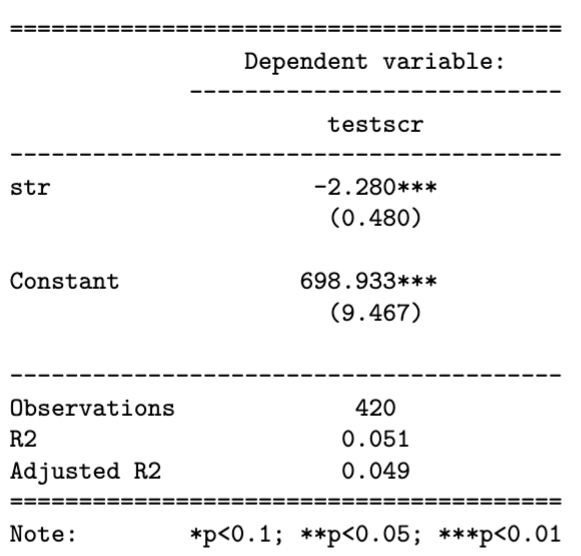
\includegraphics[scale=0.375]{reg_output_stargazer.png}
\end{column}	
\begin{column}{0.575\textwidth}
\begin{itemize} 
\item Predicted values/residuals from the fitted line: \vspace{-0.5em}
$$ \hat{testscr} = 698.93 -2.28 \cdot str $$	
\item Interpret the output
\begin{itemize}
  \item Coefficients
  \item Statistical significance \\ ($t$-stats, $p$-values) 
  \item $R^2$
\end{itemize} 
\item Exogeneity assumption:\vspace{-0.5em}
$$ E(u_i|STR_i) = E(u_i) = 0  $$
\end{itemize}
\end{column}	
\end{columns}
\end{frame}

%%%%%%%%%%%%%%%%%%%%
\begin{frame}{Omitted Variable Bias}
Consider the following linear regression model:
$$ Y = \beta_0 + \beta_1 X + u  $$

\begin{witemize}
  \item Here, $u$ captures omitted factors that impact $Y$.
  \item If $u$ is correlated with $X$, the exogeneity assumption fails and OLS estimates are biased.
  $$ \hat{\beta}_1 = \beta_1 +  \frac{Cov(X,u)}{Var(X)} $$
\item Strength and direction of bias depends on $Cov(X,u)$
\end{witemize}
\end{frame}


\begin{frame}{Omitted Variable Bias}
$$ Y = \beta_0 + \beta_1 X + u  $$
\vspace{0.1em}

Note that omitted variable bias only occurs when \underline{both} of the following are true: \\  \vspace{0.25em}
\begin{witemize}
  \item[(1)] The omitted variable is correlated with $X$
  \item[(2)] The omitted variable $\rightarrow$ Y
\end{witemize}
\end{frame}


%%%%%%%%%%%%
\begin{frame}{Omitted Variable Bias}
In our example:
$$ testscr = \beta_0 + \beta_1 str + u $$	
\vspace{0.1em}

Omitting $comp\_stu$ from this model will probably overestimate the impact of $str$. \\~\\

This is because we expect $comp\_stu$ to positively impact $testscr$ and $Cov(comp\_stu, str)<0$. \\~\\
So $comp\_stu$ being omitted leads to $Cov(str,u)<0$, hence from the OVB formula $\hat{\beta}_1<\beta_1$.
\end{frame}

%%%%%%%%%%%% 
\begin{frame}{Test Scores and Class Size}
\vspace{-0.5em}
\centering
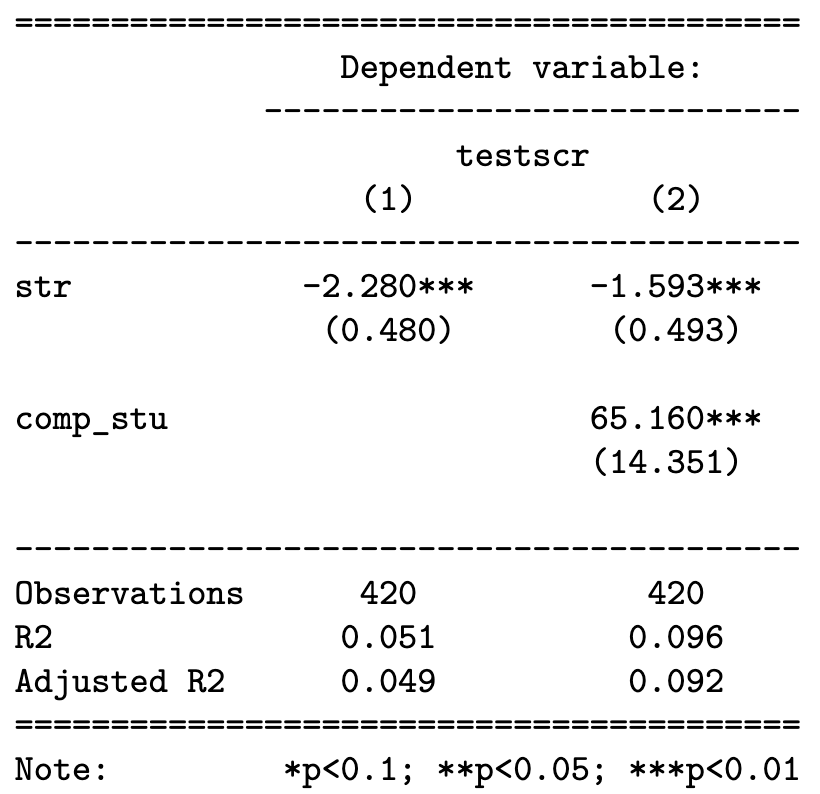
\includegraphics[scale=0.3]{reg_output_stargazer2.png}
\end{frame}


%%%%%%%%%%%%
\begin{frame}{Multiple Regression Model}
$$ Y = \beta_0 + \beta_1 X_{1} + \beta_2 X_{2} + u  $$ 
\begin{witemize}
  \item Assumptions: (1) random sample, (2) no large outliers, (3) no perfect multicollinearity, (4) $E(u | X_1, X_2)=0$
  \item Under these assumptions, $\beta_1$ captures the causal effect of $X_1$ keeping $X_2$ constant, and $\beta_2$ captures the causal effect of $X_2$ keeping $X_1$ constant. 
\end{witemize}
\end{frame}

%%%%%%%%%%%%
\begin{frame}{Control Variables}
\begin{witemize}
  \item While there are cases where we might want to evaluate the effect of both the variables, it is hard to find exogenous variables 
  \item A really good use of the multiple regression model is to instead \textit{control} for omitted variable $W$ while trying to estimate the causal effect of $X$
  $$ Y = \beta_0 + \beta_1 X + \beta_2 W + u  $$ 
\end{witemize}
\end{frame}

%%%%%%%%%%%%
\begin{frame}{Control Variables}
  $$ Y = \beta_0 + \beta_1 X + \beta_2 W + u  $$ 
  \begin{witemize}
  \item So instead of assumption (4), we can assume \textit{conditional mean independence}  $$ E(u|X,W) = E(u|W) $$
  \item The idea is that once you control for the $W$, $X$ becomes independent of $u$
  \item Under this modified assumption, we can interpret $\beta_1$ as the causal effect of $X$ while \textit{controlling} for $W$ 
\end{witemize}
\end{frame}

%%%%%%%%%%%%
\begin{frame}{Adjusted $R^2$}
$R^2$ never decreases when an explanatory variable is added \\~\\
An alternative measure called Adjusted $R^2$ 
$$ Adjusted R^2 = 1-\frac{RSS/(n-k-1)}{TSS/(n-1)} $$ 
where $k$ is the number of variables. \\~\\
$Adjusted R^2$ only rises if RSS declines by a larger percentage than the degrees
of freedom ($n-k-1$).
\end{frame}

%%%%%%%%%%%%
\begin{frame}{Dummy Variables}
What if the independent variable is a binary variable that takes two values 1 and 0?  
$$ Y = \beta_0 + \beta_1 D + u  $$ \\~\\
Taking conditional expectation (assuming exogeneity):
\begin{align*}
	E[Y | D=1] &= \beta_0 + \beta_1 \cdot 1  = \beta_0 + \red{\beta_1} \\
	E[Y | D=0] &= \beta_0 + \beta_1 \cdot 0 = \beta_0 
\end{align*}
So, $$\red{\beta_1} = E[Y | D=1]-E[Y | D=0] $$  
\end{frame}


%%%%%%%%%%%%
\begin{frame}{ACS Data: Gender Wage Gap}
\centering  \small \vspace{1.25em}

% Table created by stargazer v.5.2.3 by Marek Hlavac, Social Policy Institute. E-mail: marek.hlavac at gmail.com
% Date and time: Thu, Nov 02, 2023 - 11:46:49
\begin{tabular}{@{\extracolsep{5pt}}lc} 
\\[-1.8ex]\hline 
\hline \\[-1.8ex] 
\\[-1.8ex] & Wages \\ 
\hline \\[-1.8ex] 
 Intercept & 67,220.17$^{***}$ \\ 
  & (439.87) \\ 
  & \\ 
 Female & $-$14,661.12$^{***}$ \\ 
  & (637.27) \\ 
  & \\ 
\hline \\[-1.8ex] 
Observations & 17,578 \\ 
R$^{2}$ & 0.03 \\ 
\hline 
\hline \\[-1.8ex] 
\textit{Note:}  & \multicolumn{1}{r}{$^{*}$p$<$0.1; $^{**}$p$<$0.05; $^{***}$p$<$0.01} \\ 
\end{tabular} 
 \\ \vspace{1.5em}
\end{frame}

%%%%%%%%%%%%
\begin{frame}{Dummy Variables in Multiple Regression}
$$ Wages = \beta_0 + \beta_1 Age + \beta_2 Female +  u  $$ \\~\\
Taking conditional expectation (assuming exogeneity):
\begin{align*}
	E[Wages | Age, Female=1] &= (\beta_0+\red{\beta_2}) + \beta_1 Age
 \\
	E[Wages | Age, Female=0] &= \beta_0 + \beta_1 Age
	\end{align*} \\~\\
\end{frame}

%%%%%%%%%%%%
\begin{frame}{ACS Data: Wages and Age}
\centering  \small 
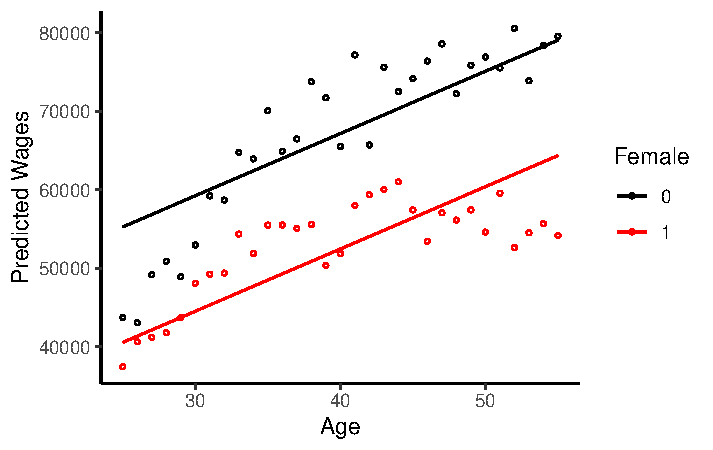
\includegraphics{./../../output/fit_gender_age.pdf} \\ \vspace{1.5em}
\end{frame}

%%%%%%%%%%%%
\begin{frame}{Interaction Terms}
We can also include interaction terms in our model as follows:
$$ Wages = \beta_0 + \beta_1 Age + \beta_2 Female + \beta_3 Female \times Age +  u  $$ \\~\\
Taking conditional expectation (assuming exogeneity):
\begin{align*}
	E[Wages | Age, Female=1] &= (\beta_0+\red{\beta_2}) + (\beta_1+\red{\beta_3}) Age
 \\
	E[Wages | Age, Female=0] &= \beta_0 + \beta_1 Age
	\end{align*} \\~\\
Now the impact of $X$ on $Y$ varies with $D$.
\end{frame}

%%%%%%%%%%%%
\begin{frame}{ACS Data: Wages and Age}
\vspace{-.5em}
\centering \small
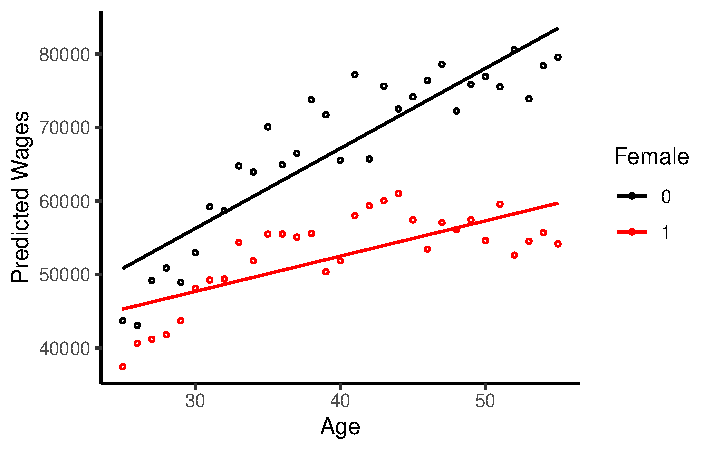
\includegraphics{./../../output/fit_gender_age_inter.pdf} \\ \vspace{1.5em}
\end{frame}

%%%%%%%%%%%%
\begin{frame}{Interaction of Two Dummy Variables}
\vspace{-1em}
$$ wages = \beta_0 + \beta_1 Female + \beta_2 Hispanic + \beta_3 Female \times Hispanic +  u  $$ \\~\\
Average wages for Non-Hispanic Males:
$$ E(wages|Hispanic=0, Female=0) = \beta_0  $$ 
Average wages for Non-Hispanic Females:
$$ E(wages|Hispanic=0, Female=1) = \beta_0 + \red{\beta_1}  $$
\end{frame}

%%%%%%%%%%%%
\begin{frame}{Interaction of Two Dummy Variables}
\vspace{-1em}
$$ wages = \beta_0 + \beta_1 Female + \beta_2 Hispanic + \beta_3 Female \times Hispanic +  u  $$ \\~\\
Average wages for Hispanic Males:
$$ E(wages|Hispanic=1, Female=0) = \beta_0 + \beta_2  $$ 
Average wages for Hispanic Females:
$$ E(wages|Hispanic=1, Female=1) = \beta_0 + \red{\beta_1} + \beta_2 + \red{\beta_3}  $$
\end{frame}

%%%%%%%%%%%%
\begin{frame}{ACS Data: Gender and Ethnicity}
\centering  \small  

% Table created by stargazer v.5.2.3 by Marek Hlavac, Social Policy Institute. E-mail: marek.hlavac at gmail.com
% Date and time: Tue, Apr 18, 2023 - 18:20:28
\begin{tabular}{@{\extracolsep{5pt}}lc} 
\\[-1.8ex]\hline 
\hline \\[-1.8ex] 
\\[-1.8ex] & Wages \\ 
\hline \\[-1.8ex] 
 Intercept & 70,179.09$^{***}$ \\ 
  & (473.52) \\ 
  & \\ 
 Female & $-$16,046.81$^{***}$ \\ 
  & (683.42) \\ 
  & \\ 
 Hispanic & $-$19,367.71$^{***}$ \\ 
  & (1,211.46) \\ 
  & \\ 
 Female X Hispanic & 8,163.75$^{***}$ \\ 
  & (1,788.04) \\ 
  & \\ 
\hline \\[-1.8ex] 
Observations & 17,578 \\ 
R$^{2}$ & 0.05 \\ 
\hline 
\hline \\[-1.8ex] 
\textit{Note:}  & \multicolumn{1}{r}{$^{*}$p$<$0.1; $^{**}$p$<$0.05; $^{***}$p$<$0.01} \\ 
\end{tabular} 
 \\ \vspace{1.5em}
\end{frame}

%%%%%%%%%%%%
\begin{frame}{Fitting a Line}
Linear relationship:
$$ \hat{Y} = \hat{\beta}_0 + \hat{\beta}_1 X   $$

Take the derivative:
$$ \frac{d \hat{Y}}{dX} = \hat{\beta}_1 \rightarrow d \hat{Y} = \hat{\beta}_1 dX  $$ \\~\\

Can think of $d$ as `change in':
One unit change in $X$, associated with $\beta_1$ units change in $Y$. \\~\\
Impact of $X$ on $Y$ constant with $X$. \\~\\
\end{frame}

%%%%%%%%%%%%
\begin{frame}{Fitting a Curve}
Quadratic relationship:
$$ \hat{Y} = \hat{\beta}_0 + \hat{\beta}_1 X + \hat{\beta}_2 X^2   $$

Take the derivative:
$$ \frac{d \hat{Y}}{dX} = \hat{\beta}_1 + 2 \hat{\beta}_2 X $$ \\~\\

Now the impact of $X$ on $Y$ changes with $X$. \\~\\
Remember: Derivative captures the slope of the tangent line.

\end{frame}

%%%%%%%%%%%%
\begin{frame}{ACS Data: Wages and Age}
\centering \vspace{-2em}
$$ \hat{wage} = -52207 + 4775.64 \cdot age -49.493 \cdot age^2   $$
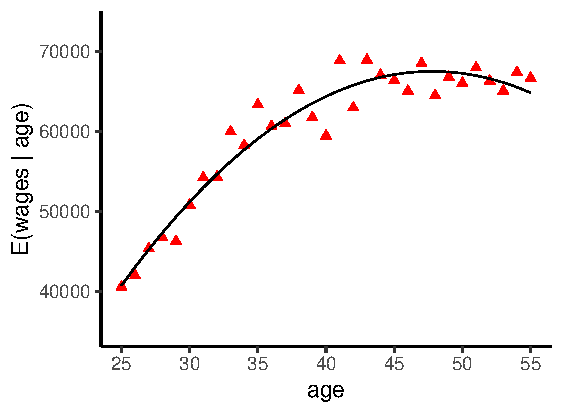
\includegraphics{./../../output/scatter_age_wage_qfit.pdf}
\end{frame}

%%%%%%%%%%%%
\begin{frame}{Log Functional Forms}
\vspace{-0.5em}
\begin{witemize}
  \item Log-transformation leads to interpretation of regression coefficients in \% changes than unit changes which can sometimes be more informative 
  \item Can think of change in log of X as the relative change in X with respect to its original value
  $$ \frac{d}{dX} \log(X) = \frac{1}{X} \rightarrow d \log(X) = \frac{d X}{X} $$
  In which case $100 \times d\log(X)$ represents \% change in $X$
\end{witemize}
\end{frame}


%%%%%%%%%%%%
\begin{frame}{Log Functional Forms: Interpretation}
Three possible models: \\~\\
\begin{enumerate}
  \item Level-Log: $ \quad \hat{Y} = \hat{\beta}_0 +  \hat{\beta}_1 log(X) $ \\~\\
  \item Log-Level: $ \quad \hat{log}(Y) = \hat{\beta}_0 +  \hat{\beta}_1 X $ \\~\\
  \item Log-Log: $ \quad \log(\hat{Y}) = \hat{\beta}_0 +  \hat{\beta}_1 \log(X) $
\end{enumerate}
\end{frame}

%%%%%%%%%%%%
\begin{frame}{Log-Level Model}
\centering \small \vspace{-0.5em}

% Table created by stargazer v.5.2.3 by Marek Hlavac, Social Policy Institute. E-mail: marek.hlavac at gmail.com
% Date and time: Tue, Apr 18, 2023 - 13:49:03
\begin{tabular}{@{\extracolsep{5pt}}lc} 
\\[-1.8ex]\hline 
\hline \\[-1.8ex] 
\\[-1.8ex] & Log Wages \\ 
\hline \\[-1.8ex] 
 Intercept & 10.31$^{***}$ \\ 
  & (0.02) \\ 
  & \\ 
 Age & 0.01$^{***}$ \\ 
  & (0.001) \\ 
  & \\ 
\hline \\[-1.8ex] 
Observations & 17,578 \\ 
R$^{2}$ & 0.03 \\ 
\hline 
\hline \\[-1.8ex] 
\textit{Note:}  & \multicolumn{1}{r}{$^{*}$p$<$0.1; $^{**}$p$<$0.05; $^{***}$p$<$0.01} \\ 
\end{tabular} 
 \\ \vspace{1.5em}
\normalsize \textit{1 year increase in age leads to 1\% increase in predicted wages.} 
\end{frame}


%%%%%%%%%%%%
\begin{frame}{Log-Log Model}
\centering \small \vspace{-0.5em}

% Table created by stargazer v.5.2.3 by Marek Hlavac, Social Policy Institute. E-mail: marek.hlavac at gmail.com
% Date and time: Tue, Apr 18, 2023 - 13:49:03
\begin{tabular}{@{\extracolsep{5pt}}lc} 
\\[-1.8ex]\hline 
\hline \\[-1.8ex] 
\\[-1.8ex] & Log Wages \\ 
\hline \\[-1.8ex] 
 Intercept & 8.99$^{***}$ \\ 
  & (0.08) \\ 
  & \\ 
 Log Age & 0.49$^{***}$ \\ 
  & (0.02) \\ 
  & \\ 
\hline \\[-1.8ex] 
Observations & 17,578 \\ 
R$^{2}$ & 0.03 \\ 
\hline 
\hline \\[-1.8ex] 
\textit{Note:}  & \multicolumn{1}{r}{$^{*}$p$<$0.1; $^{**}$p$<$0.05; $^{***}$p$<$0.01} \\ 
\end{tabular} 
 \\ \vspace{1.5em}
\normalsize \textit{1\% increase in age leads to 0.49\% increase in predicted wages.} 
\end{frame}

%%%%%%%%%%%%%%
\begin{frame}{A Few Last Words}
\vspace{0.7em}
\large \centering
Good luck and take care! \\~\\
Thanks for a great
semester! \\~\\
Have a great break, and don’t be a stranger!
\end{frame}


\end{document}